\documentclass{article}

\title{Intro To Artificial Intelligence - Exercise 2}
\author{Eran Ston (206704512) and Oded Vaalany (208230474)}
\date{\today}
\usepackage{amsmath} % for advanced math equations
\usepackage{amssymb} % for additional math symbols
\usepackage{amsfonts} % for math fonts
\usepackage{mathtools} % for additional math tools
\usepackage{amsthm} % for theorem environments
\usepackage[margin=1.5cm]{geometry}
\usepackage{enumitem}
\begin{document}

\maketitle

\section{CNF}
\begin{tabular}{ccccccccc}
    $P$ & $Q$  & $\neg Q$ & $P \lor Q$ & $P \land Q$ & $\neg Q \lor P$ & $\neg Q \land P$ & $Q \Rightarrow P$ & $P \iff Q$\\
    true&true&false&true&true&true&false&true&true\\
    true&false&true&true&false&true&true&true&false\\
    false&true&false&true&false&false&false&false&false\\
    false&false&true&false&false&true&false&true&true\\
\end{tabular}\\
so we can conclude that:
\begin{enumerate}
    \item $Q \Rightarrow P \equiv \neg Q \lor P$
    \item $Q \iff P \equiv P \Rightarrow Q \land P \Leftarrow Q $
    \item $P \iff Q \equiv Q \Rightarrow P \land P \Rightarrow Q  \equiv (\neg Q \lor P) \land (\neg P \lor Q)$
    \item $\neg \neg P \equiv P$
\end{enumerate}
convert each of the following formulas to CNF:
\subsection{1. $(P \Rightarrow \neg Q) \iff R$}
\begin{equation}
    Q \Rightarrow P \equiv \neg Q \lor P
\end{equation}
\subsection{2. $\neg (P \land \neg Q) \Rightarrow \neg R \lor \neg Q$}
\begin{equation}
    \begin{aligned}
        (P \Rightarrow \neg Q) \iff R &\overbrace{\equiv}^{\text{rule (2)}} (P \Rightarrow \neg Q) \Rightarrow R \land (P \Rightarrow \neg Q) \Leftarrow R\\
        &\overbrace{\equiv}^{\text{rule (1)}} (\neg (P \Rightarrow \neg Q) \lor R ) \land (( P \Rightarrow \neg Q) \lor \neg R)\\
        &\overbrace{\equiv}^{\text{rule (1)}} (\neg (\neg P \lor \neg Q) \lor R ) \land ((\neg P \lor \neg Q) \lor \neg R)\\
        &\overbrace{\equiv}^{\text{De Morgan}} ((  P \land  Q) \lor R) \land (\neg P \lor \neg Q \lor \neg R)\\
        &\overbrace{\equiv}^{\text{Distribution}} ( P \lor R) \land (  Q \lor R) \land  (\neg P \lor \neg Q \lor \neg R)
    \end{aligned}
\end{equation}
\subsection{3. $\neg (P \land  \neg Q) \Rightarrow (\neg R\lor \neg Q)$}
\begin{equation}
    \begin{aligned}
        \neg (P \land \neg Q) \Rightarrow \neg R \lor \neg Q &\overbrace{\equiv}^{\text{rule (1)}} (\neg(\neg(P \land \neg Q)) \lor (\neg R \lor \neg Q))\\
        &\overbrace{\equiv}^{\text{rule (4)}} ((P \land \neg Q) \lor \neg R \lor \neg Q)\\
        &\overbrace{\equiv}^{\text{Distribution}} (P \lor \neg R \lor \neg Q) \land (\neg Q \lor \neg R)
    \end{aligned}
\end{equation}
\subsection{4. $\neg (P \iff \neg Q) \Rightarrow R$}
\begin{equation}
    \begin{aligned}
        \neg (P \iff \neg Q) \Rightarrow R &\overbrace{\equiv}^{\text{rule (3)}} \neg ((\neg P \lor \neg Q) \land (Q \lor P)) \Rightarrow R\\
        &\overbrace{\equiv}^{\text{rule (1)}} \neg (\neg(( \neg P \lor \neg Q) \land  (Q \lor P))) \lor R\\
        &\overbrace{\equiv}^{\text{rule (4)}} (( \neg P \lor \neg Q) \land  (Q \lor P)) \lor R\\
        &\overbrace{\equiv}^{\text{Distribution}} (( \neg P \lor \neg Q) \lor R) \land ( (Q \lor P) \lor R)\\
        &\overbrace{\equiv}^{\text{}} ( \neg P \lor \neg Q \lor R) \land ( Q \lor P \lor R)\\
    \end{aligned}
\end{equation}
\subsection{5. $\neg (P \Rightarrow (\neg R \lor \neg Q)) \Rightarrow \neg R$}
\begin{equation}
    \begin{aligned}
        \neg (P \Rightarrow (\neg R \lor \neg Q)) \Rightarrow \neg R &\overbrace{\equiv}^{\text{rule (1)}} \neg (\neg P \lor \neg R \lor \neg Q) \Rightarrow \neg R\\
        &\overbrace{\equiv}^{\text{rule (1)}} \neg (\neg (\neg P \lor \neg R \lor \neg Q)) \lor \neg R\\
        &\overbrace{\equiv}^{\text{rule (4)}} \neg P \lor \neg R \lor \neg Q \lor \neg R\\
        &\overbrace{\equiv}^{\text{rule (4)}} \neg P \lor \neg R \lor \neg Q \lor \neg R\\
        &\overbrace{\equiv}^{\text{rule (4)}} \neg P \lor \neg R \lor \neg Q \lor \neg R
    \end{aligned}
\end{equation}


\section{Resolution}

\subsection{Given G = Nitay carries an umbrella}
Let's define the following predicates:
\begin{itemize}
    \item P = Nitay carries an umbrella
    \item R = If it rains
    \item W = Nitay dosen't get wet
\end{itemize}
So we can write the given statement as:
\begin{enumerate}
    \item $R \Rightarrow P \equiv \neg R \lor P$ 
    \item $P \Rightarrow W \equiv \neg P \lor W$
    \item $\neg R \Rightarrow W \equiv R \lor W$
    \item $ W$
    \item G = $P$
\end{enumerate}
Now we can start the algorithm, where KB=$(\neg R \lor P) \land (\neg P \lor W) \land (R \lor W) \land W$ and $\alpha =  P$\\
\begin{enumerate}
    \item we will define C = $KB \land \neg P \equiv \{(\overline R + P),(\overline P + W),(R + W),W,\overline P\}$ 
    \item we will define new = $\emptyset$
    \item forall $C_i, C_j$ in C: (we will write only paris that have a resolution)
    \begin{enumerate}
        \item $(\overline R + P)(\overline P + W)$ Resolution: $\overline R + W$
        \item $(\overline R + P)(R + W)$ Resolution: $\overline P + W$
        \item $(\overline R + P)(\overline P)$ Resolution: $\overline R$
    \end{enumerate}
    \item new = $\{(\overline P + W ),(\overline R + W),(\overline R)\}$
    \item new $\not\subset$ C
    \item C = C $\cup$ new $\equiv \{(\overline R + P) , (R + W), W,(\overline P + W ),(\overline R + W),(\overline R), \overline P\}$
    \item forall $C_i, C_j$ in C:
    \begin{enumerate}
        \item $(\overline R + P)(R + W)$ Resolution: $P+W $
        \item $(\overline R + P)(\overline P + W)$ Resolution: $\overline R +W $
        \item $(\overline R + P)(\overline P) $ Resolution: $\overline R$
        \item $(R+W)(\overline R + W)$ Resolution: $W$
        \item $(R+W)(\overline R)$ Resolution: $W$
    \end{enumerate}
    \item new = $\{(P+W),(\overline R + W),\overline R ,W\}$
    \item new $\not\subset$ C
    \item C = C $\cup$ new $\equiv \{(P+W),(\overline R + P) , (R + W), W,(\overline P + W ),(\overline R + W),(\overline R), \overline P\}$
    \item for all $C_i, C_j$ in C:
    \begin{enumerate}
        \item $(P+W)(\overline P + W)$ Resolution: $W$
        \item $(P+W)\overline P$ Resolution: $W$
        \item $(\overline R + P)(R + W)$ Resolution: $P+W $
        \item $(\overline R + P)(\overline P + W)$ Resolution: $\overline R +W $
        \item $(\overline R + P)(\overline P) $ Resolution: $\overline R$
        \item $(R+W)(\overline R + W)$ Resolution: $W$
        \item $(R+W)(\overline R)$ Resolution: $W$
    \end{enumerate}
    \item new = $\{W,(P+W),(\overline R + W),\overline R\}$
    \item since new $\subset$ C we will return false
\end{enumerate}
We dosn't recived a contradiction, so we can conclude that Nitay carries an umbrella.

\subsection{}
First we will define the following predicates:
\begin{itemize}
    \item $Z$: animals that make noise at night
    \item $N$: Its night 
    \item $D$: Have dog 
    \item $C$: Have cat
    \item $M$: Have mice
    \item $P$: Struggling to fall asleep
    \item $A$: Amit 
\end{itemize}
So we can write the given statement as:
\begin{enumerate}
    \item All hounds (dogs) bark at night $\equiv D \Rightarrow Z$
    \item If you have a cat, you don’t have mice $\equiv C \Rightarrow \neg M$
    \item If you have problems falling a sleep you don’t keep animals that make sound at night $\equiv P \Rightarrow \neg Z$
    \item Amit has either a dog or a cat $A(C\lor D)$
    \item G = If Amit have problems falling a sleep, then Amit has no mice $ \equiv A \land P \Rightarrow \neg M \land A \equiv \neg A + \neg P + \neg M $
\end{enumerate}
Now we can start the algorithm, where KB=$\{(\overline D + Z),(\overline  C + \overline  M),( \overline  P + \overline  Z),A,(C + D)\}$ and $\alpha = \neg M \lor \neg A \lor \neg P$\\
\begin{enumerate}
    \item we will define C = $KB \land \neg \alpha \equiv \{(\overline D + Z),(\overline  C + \overline  M),( \overline  P + \overline  Z),A,(C + D),M,P\}$
    \item new = $\emptyset$
    \item forall $C_i, C_j$ in C: (we will write only paris that have a resolution)
    \begin{enumerate}
        \item $(\overline D + Z)(\overline P + \overline Z)$ Resolution: $\overline D + \overline P$
        \item $(\overline D + Z)(C + D)$ Resolution: $Z + C$
        \item $(\overline C + \overline  M)(C+D)$ Resolution: $\overline  M + P$ 
        \item $(\overline C + \overline  M)(M)$ Resolution: $\overline  C$ 
        \item $(\overline P + \overline Z)P$ Resolution: $\overline Z$
    \end{enumerate}
    \item new = $\{\overline D + \overline P, Z + C, \overline M + P, \overline C, \overline Z\}$
    \item new $\not\subset$ C
    \item C = C $\cup$ new $\equiv \{(\overline D + Z),(\overline  C + \overline  M),( \overline  P + \overline  Z),A,(C + D),M,P,(\overline D + \overline P), (Z + C), (\overline M + P), \overline C, \overline Z\}$
    \item new = $\emptyset$
    \item forall $C_i, C_j$ in C: (we will write only paris that have a resolution)
    \begin{enumerate}
        \item $(\overline D + Z)(\overline Z)$ Resolution: $\overline D$
        \item $(\overline C + \overline M)(Z+C)$ Resolution $\overline M + Z$
        \item $(\overline P + \overline Z)(Z+C)$ Resolution: $\overline P + C$
        \item $(\overline P + \overline Z)(\overline M + P)$ Resolution: $\overline Z + \overline M$
        \item $(C+D)(\overline D + \overline P)$ Resolution: $C + \overline P$
        \item $(C+D)\overline C$ Resolution: $D$
        \item $(M)(\overline M + P)$ Resolution: $P$
        \item $P(\overline D + \overline P)$ Resolution: $\overline D$
        \item $(\overline D + \overline P)(\overline M + P)$ Resolution: $\overline D + \overline M $
        \item $(Z+C)\overline Z$ Resolution: $C$
        \item $(Z+C)\overline C$ Resolution: $Z$
    \end{enumerate}
    \item new = $\{(\overline M + Z), (\overline P + C), (\overline Z + \overline M), (C + \overline P), D, P, \overline D, (\overline D + \overline M), C, Z\}$
    \item new $\not\subset$ C
    \item C = C $\cup$ new 
    \item forall $C_i, C_j$ in C: (we will write only paris that have a resolution)
    \begin{enumerate}
        \item $\overline D \cdot D$ Resolution: $\emptyset$
        \item we will return True
    \end{enumerate}
\end{enumerate}
We received a contradiction, so we can conclude that if Amit has problems to sleep at night so amit has no mice.


\section{DPLL Algorithm}
given the following CNF formula: $(\overline A +B)(\overline C + D)(\overline E + \overline F)(F + \overline E + B)$\\
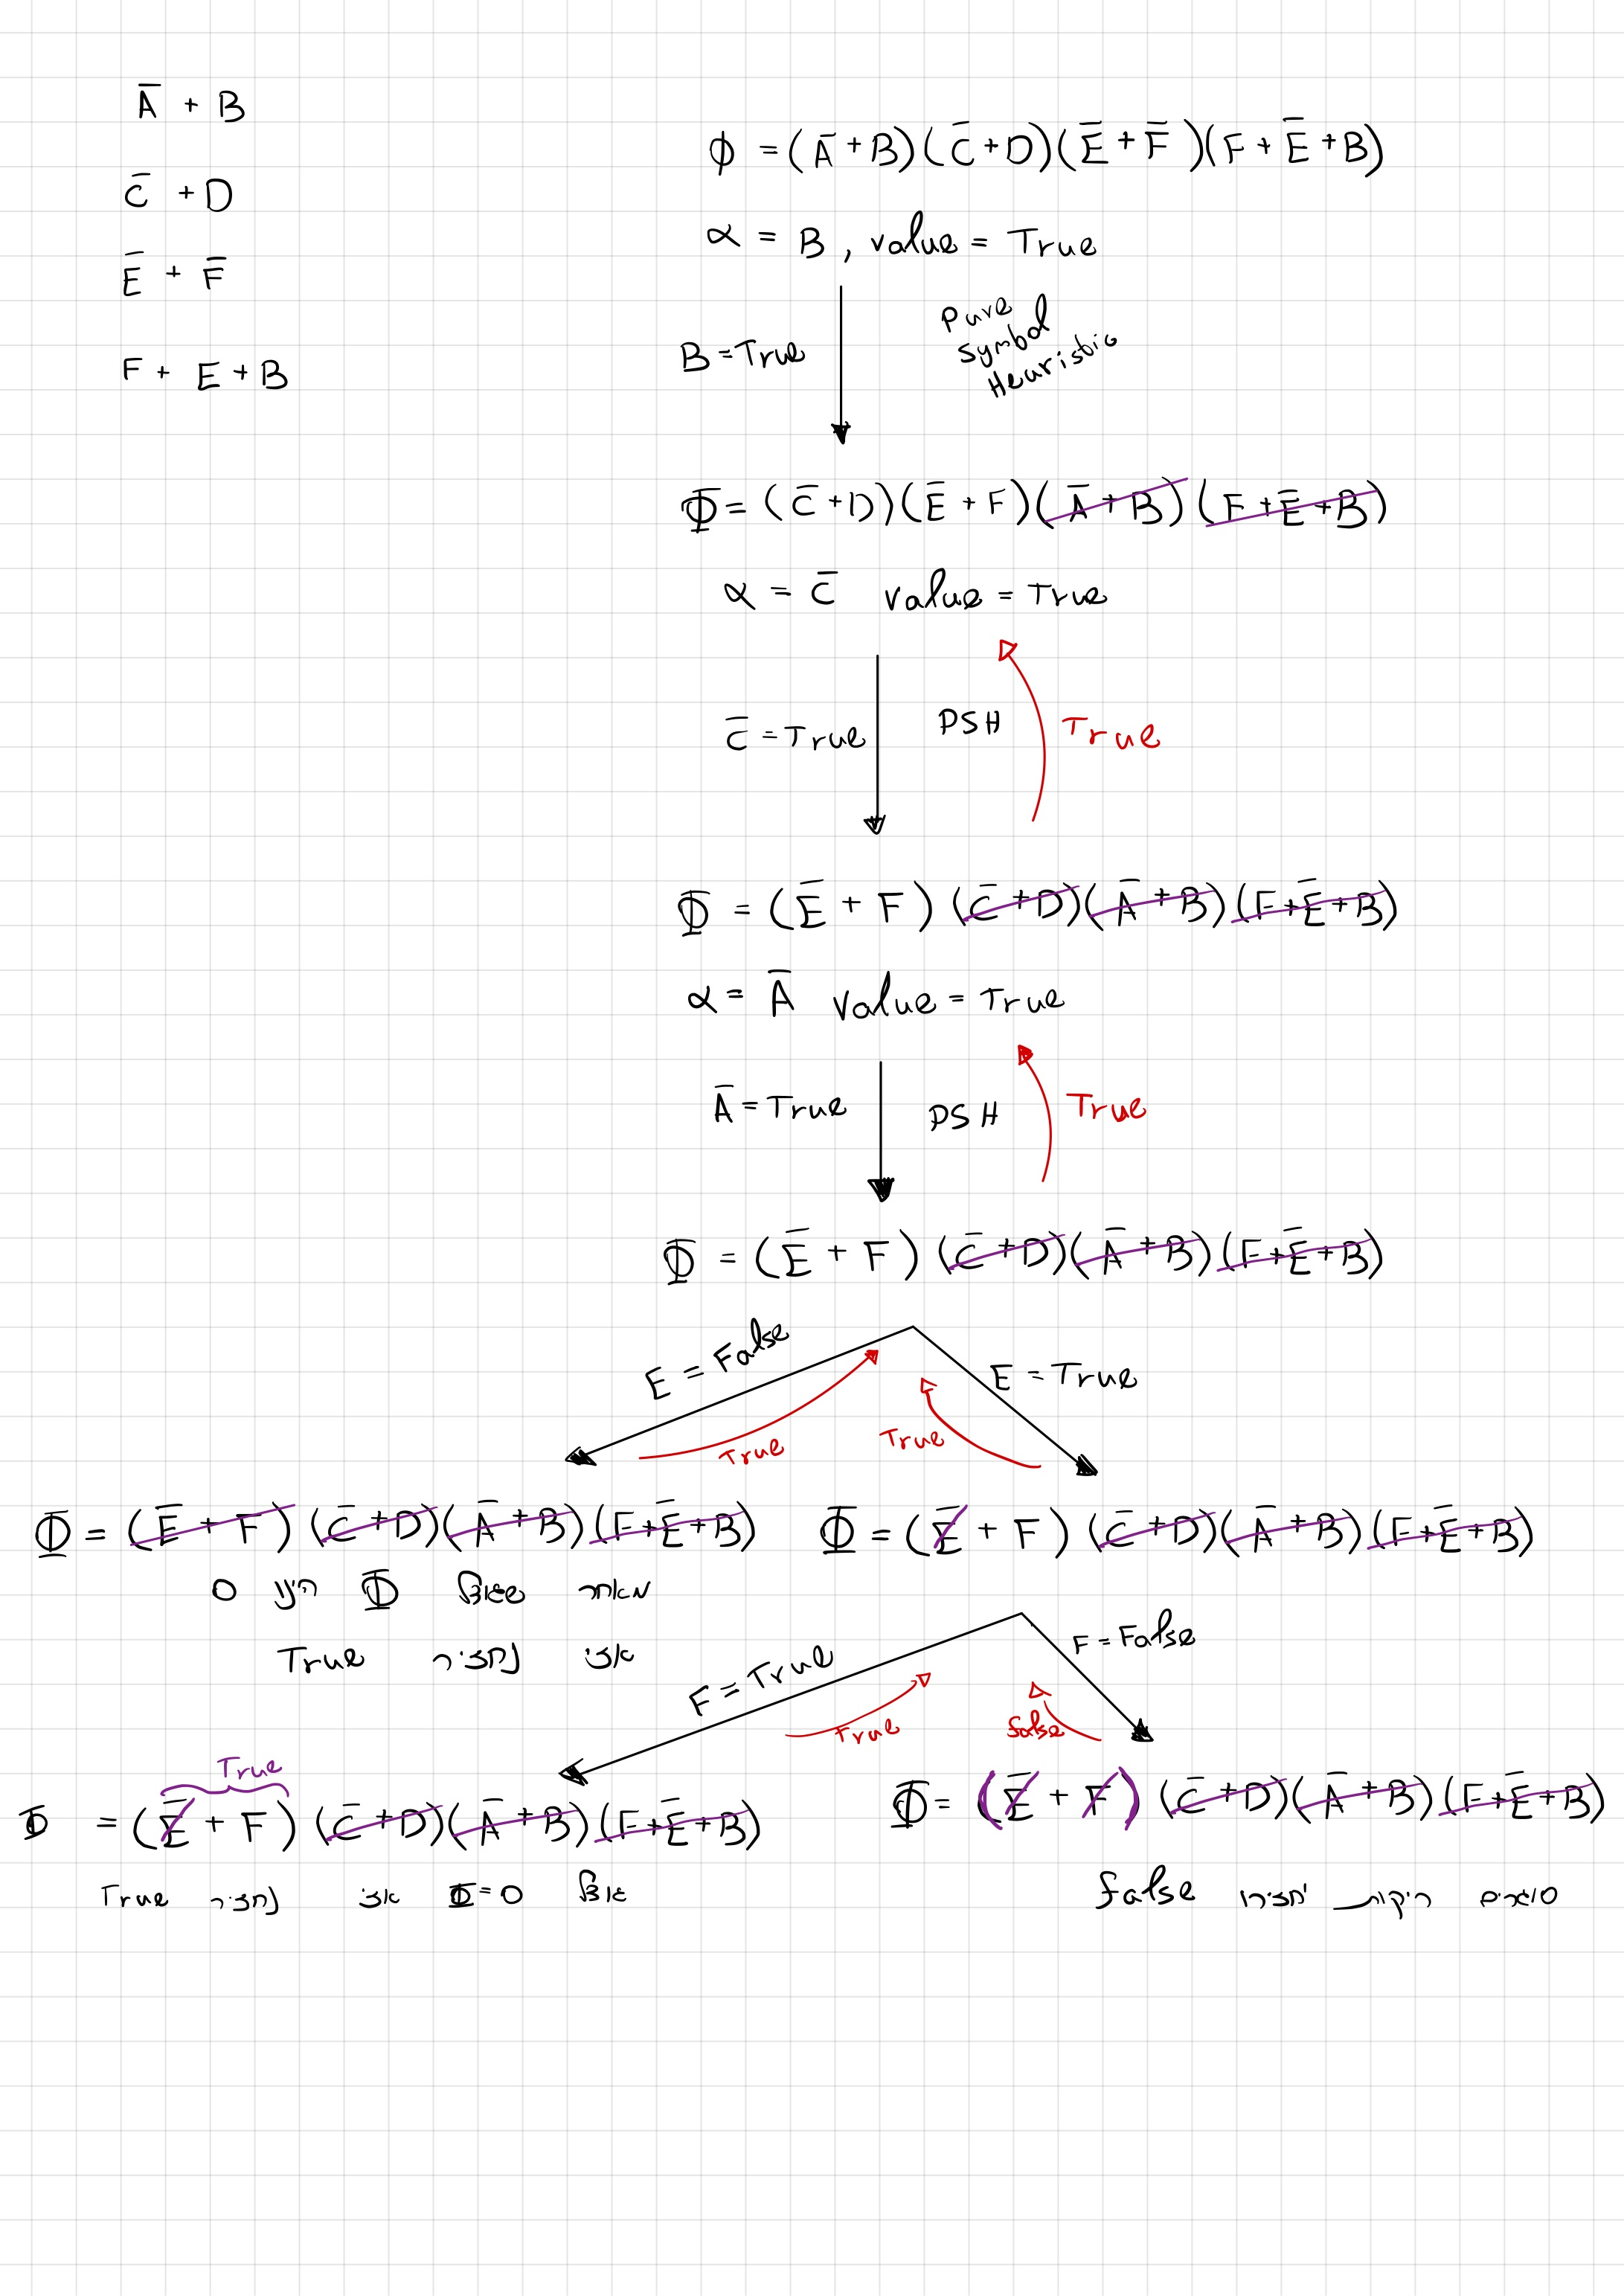
\includegraphics[width=0.8\textwidth]{DPLL.jpg}\\
% \begin{figure}[ht]
%     \centering
%     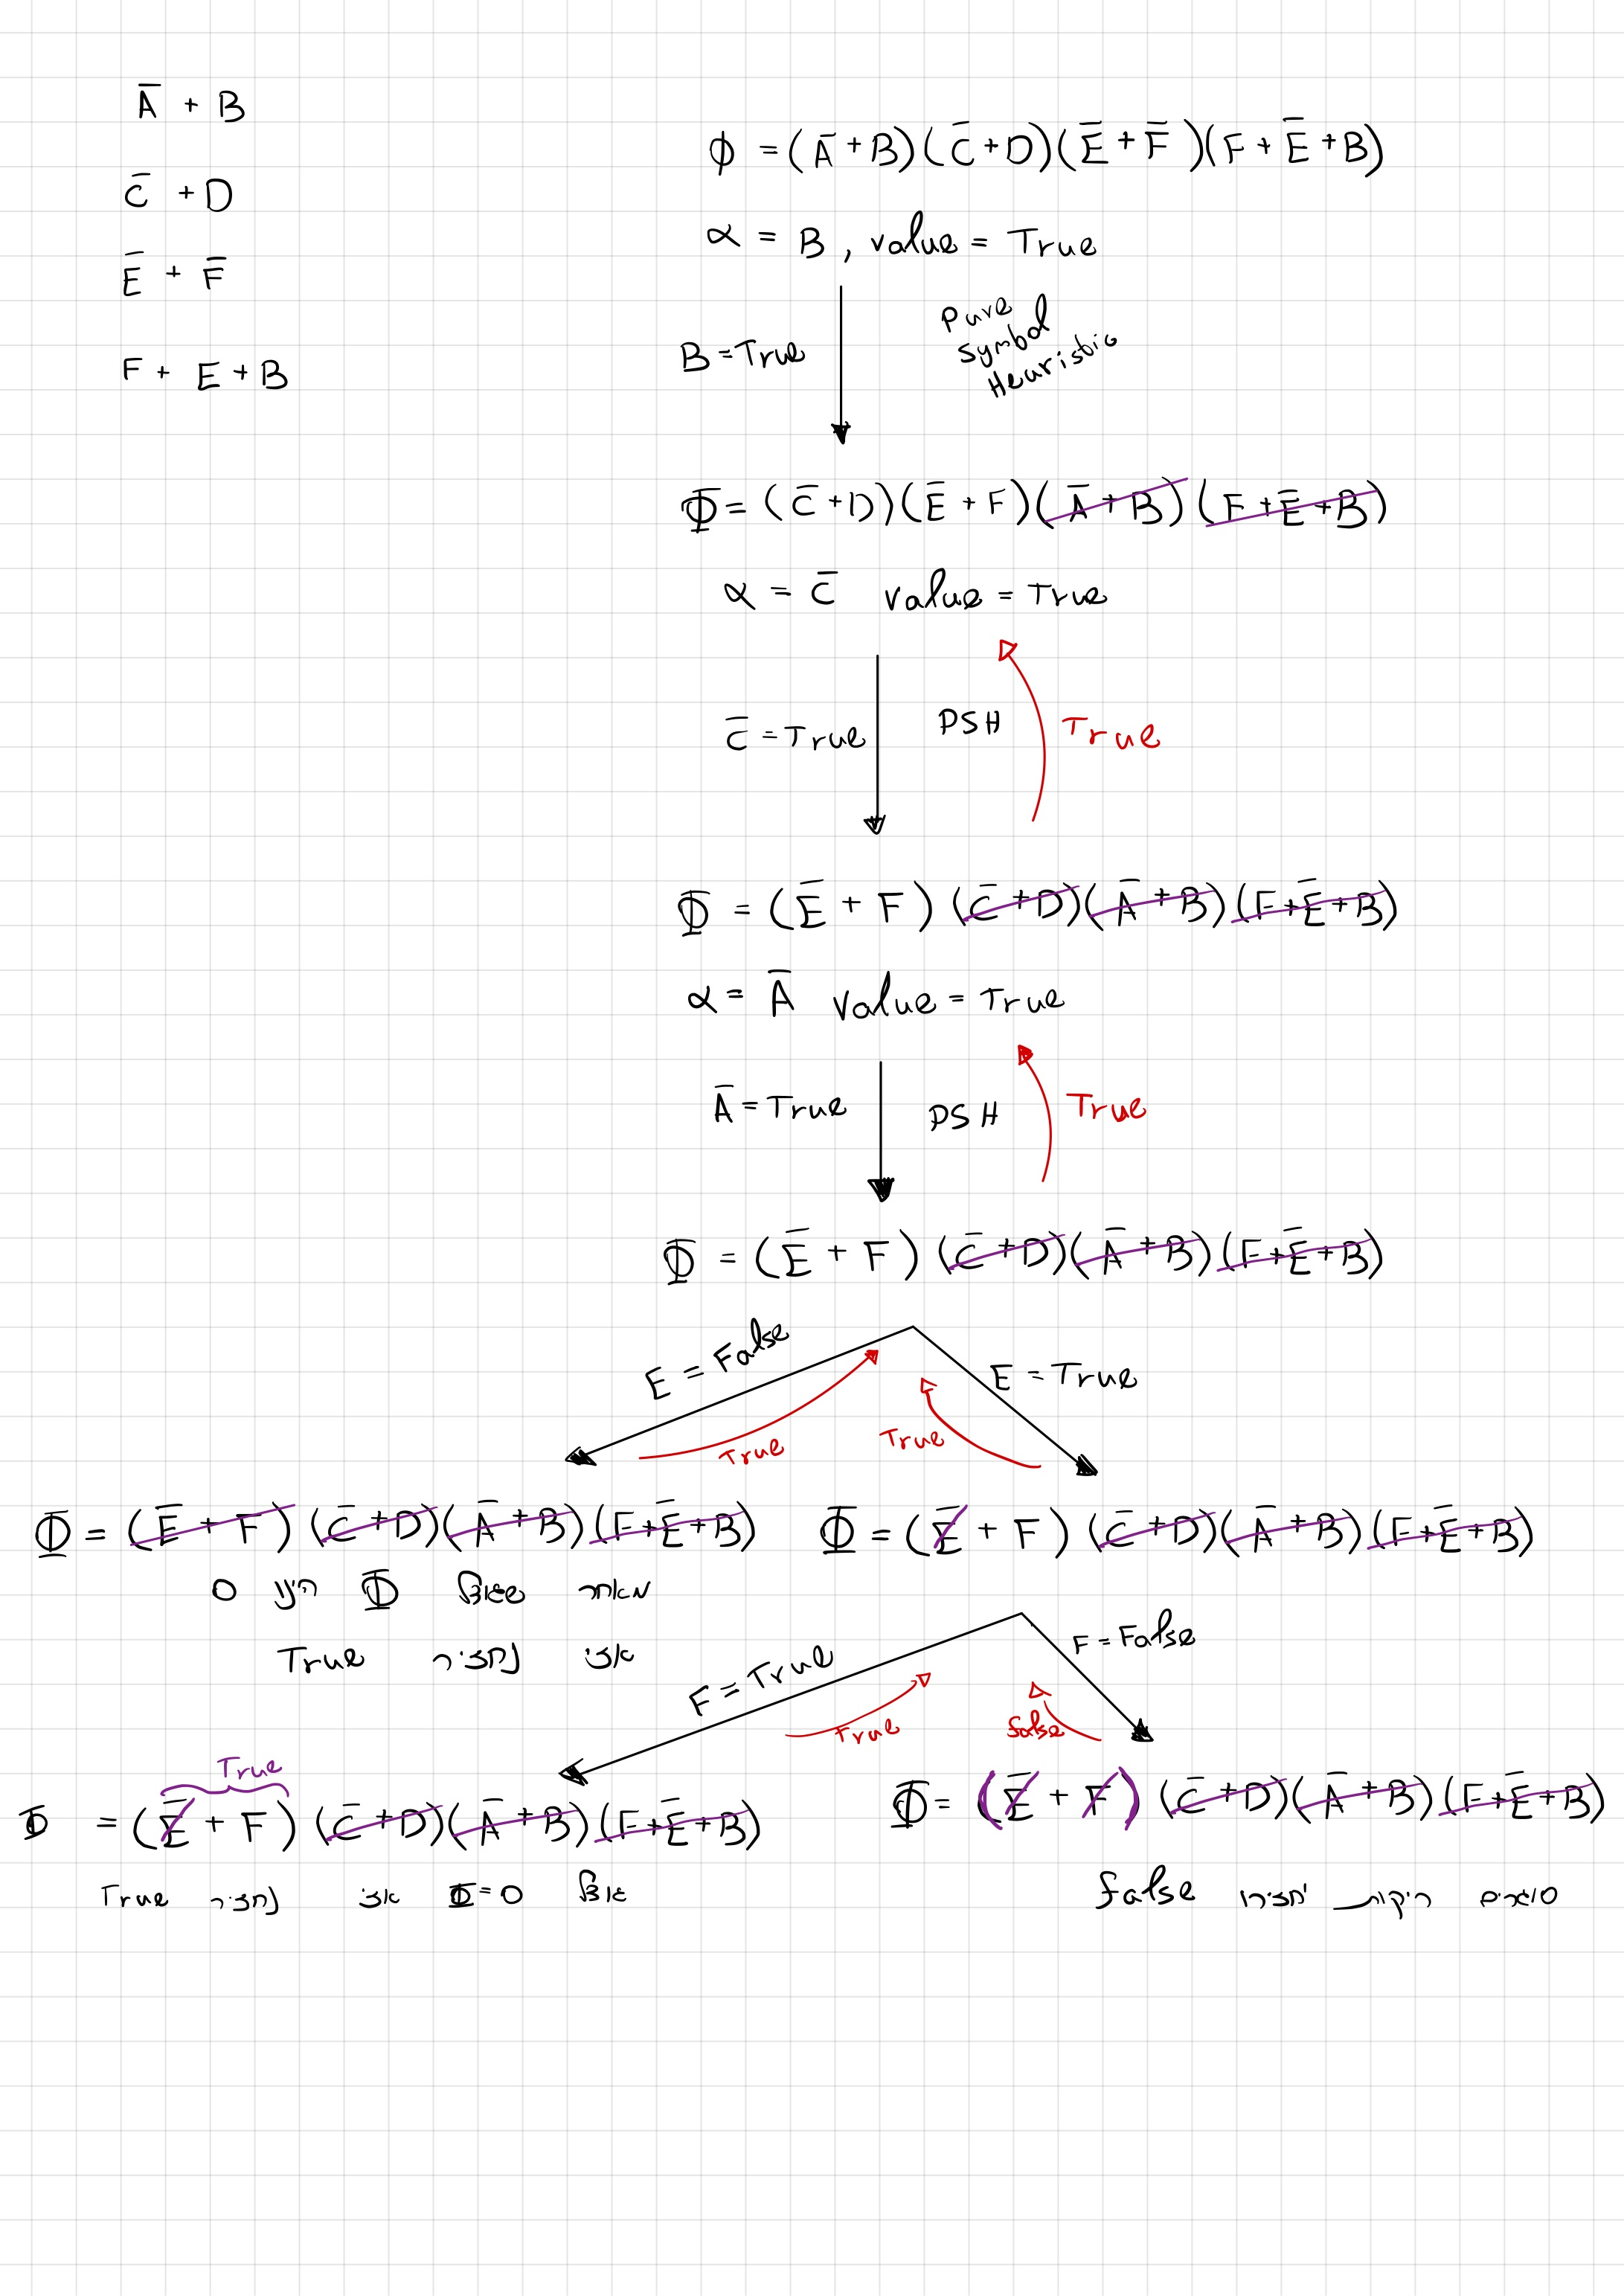
\includegraphics[width=0.8\textwidth]{DPLL.jpg}
%     \caption{Our hand written DPLL algorithm}
%     \label{fig:your_image}
% \end{figure}\\

We can see that the algorithm is working correctly and we can conclude that the formula is satisfiable.
One of the optional Models is: $B = Ture \land C = False \land A = False \land E = False \land F = True$\\
- If on the Third call we could define E as a pure symbol, we could have finished the algorithm in 3 steps. we wasn't sure so we decided to take the long way.

\end{document}